\begin{tcolorbox}[title=Especificaciones de la VM]
    \begin{itemize}
        \item Sistema operativo: Kali Linux
        \item Memoria Base: 4096 MB
        \item Núcleos: 4
        \item Versión: 2025.4
    \end{itemize}
\end{tcolorbox}

En general todo el proceso de este reporte ocurrió dentro de la misma terminal, con la excepción de la terminal de
la máquina Host.

\section{Algoritmos KEX en la VM de Kali Linux}

\begin{figure}[H]
    \centering
    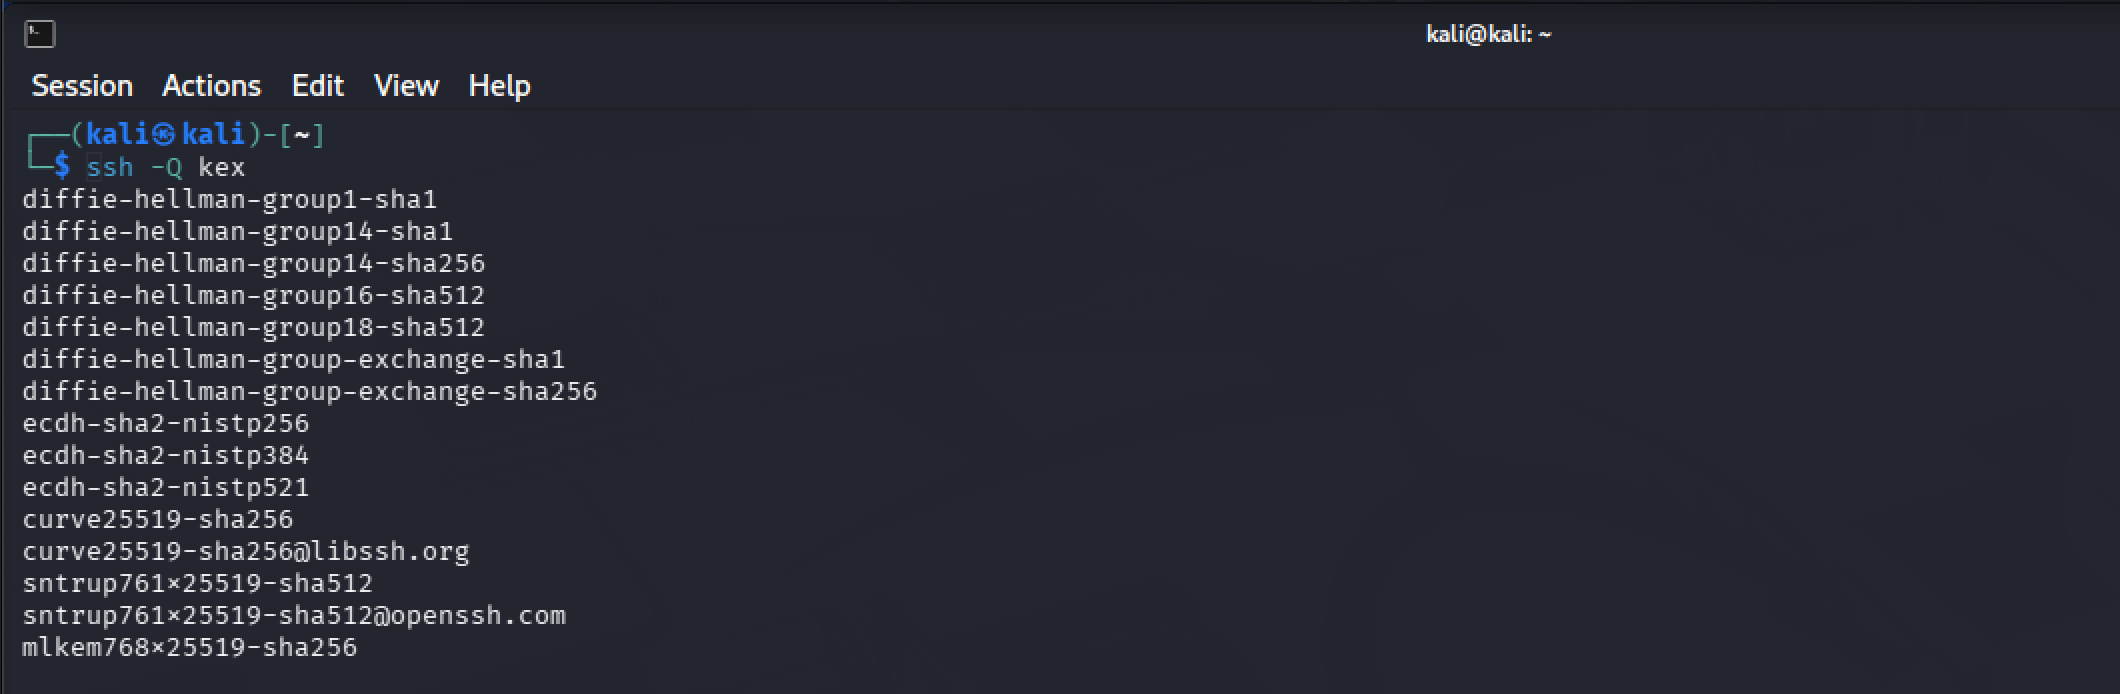
\includegraphics[width=0.8\textwidth]{imagenes/ssh-q-kex.png}
    \caption{Algoritmos KEX en la VM de Kali Linux.}
    \label{fig:ssh-q-kex}
\end{figure}

Vemos que hay 15 algoritmos disponibles en la VM, incluyendo los 5 mencionados en la presentación vista en clase. Como se
indica en la anterior, no se recomienda usar \texttt{diffie-hellman-group1-sha1} y \texttt{diffie-hellman-group14-sha1}.

\section{Instalación y configuración de OpenSSH en la VM de Kali Linux}

\begin{figure}[H]
    \centering
    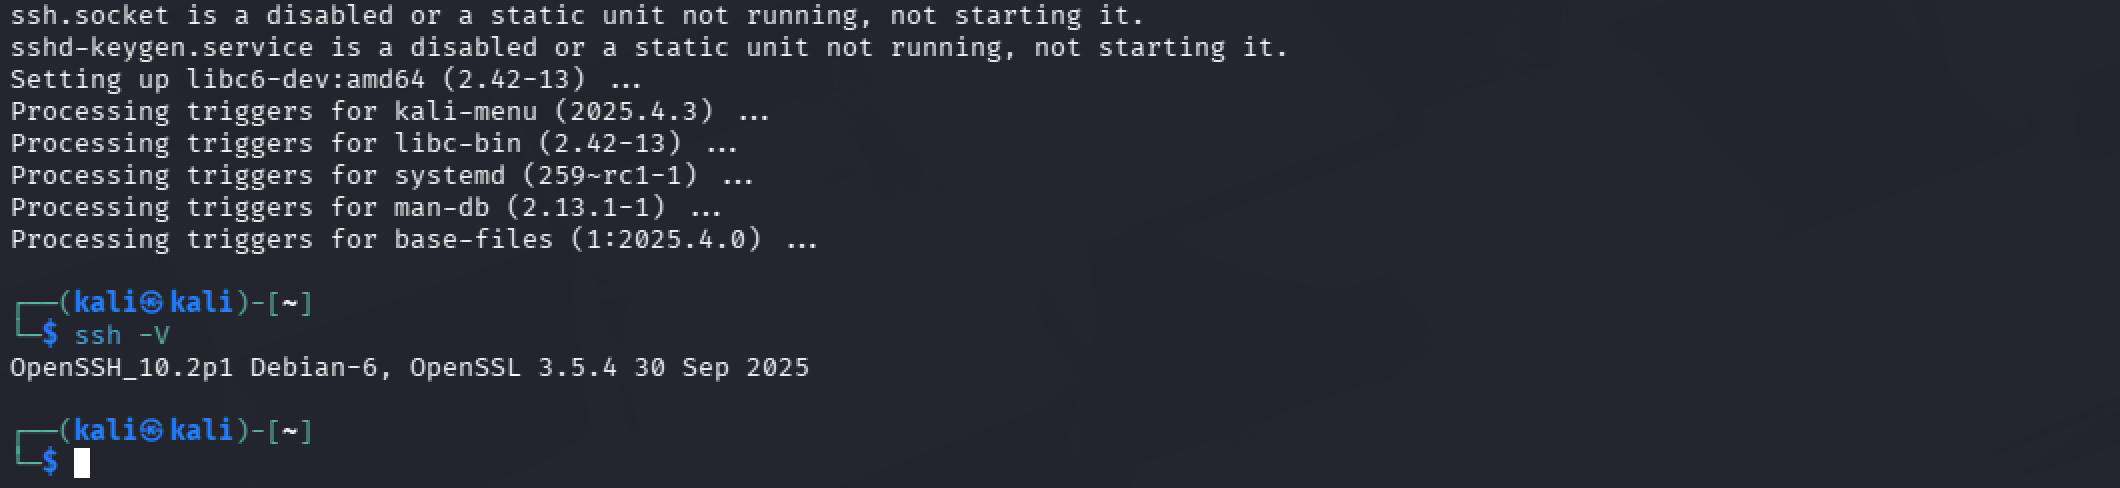
\includegraphics[width=0.85\textwidth]{imagenes/install_openssh.png}
    \caption{Instalación de OpenSSH en la VM de Kali Linux.}
    \label{fig:install-openssh}
\end{figure}

Nótese que en la imágen no se muestra todo el proceso de instalación, pero se puede observar que se ha instalado el
paquete \texttt{openssh-server} de manera correcta pues al hacer \texttt{ssh -V} se muestra la versión instalada, que
en este caso es la 10.2p1.

\section{Habilitación del servicio SSH}

\begin{figure}[H]
    \centering
    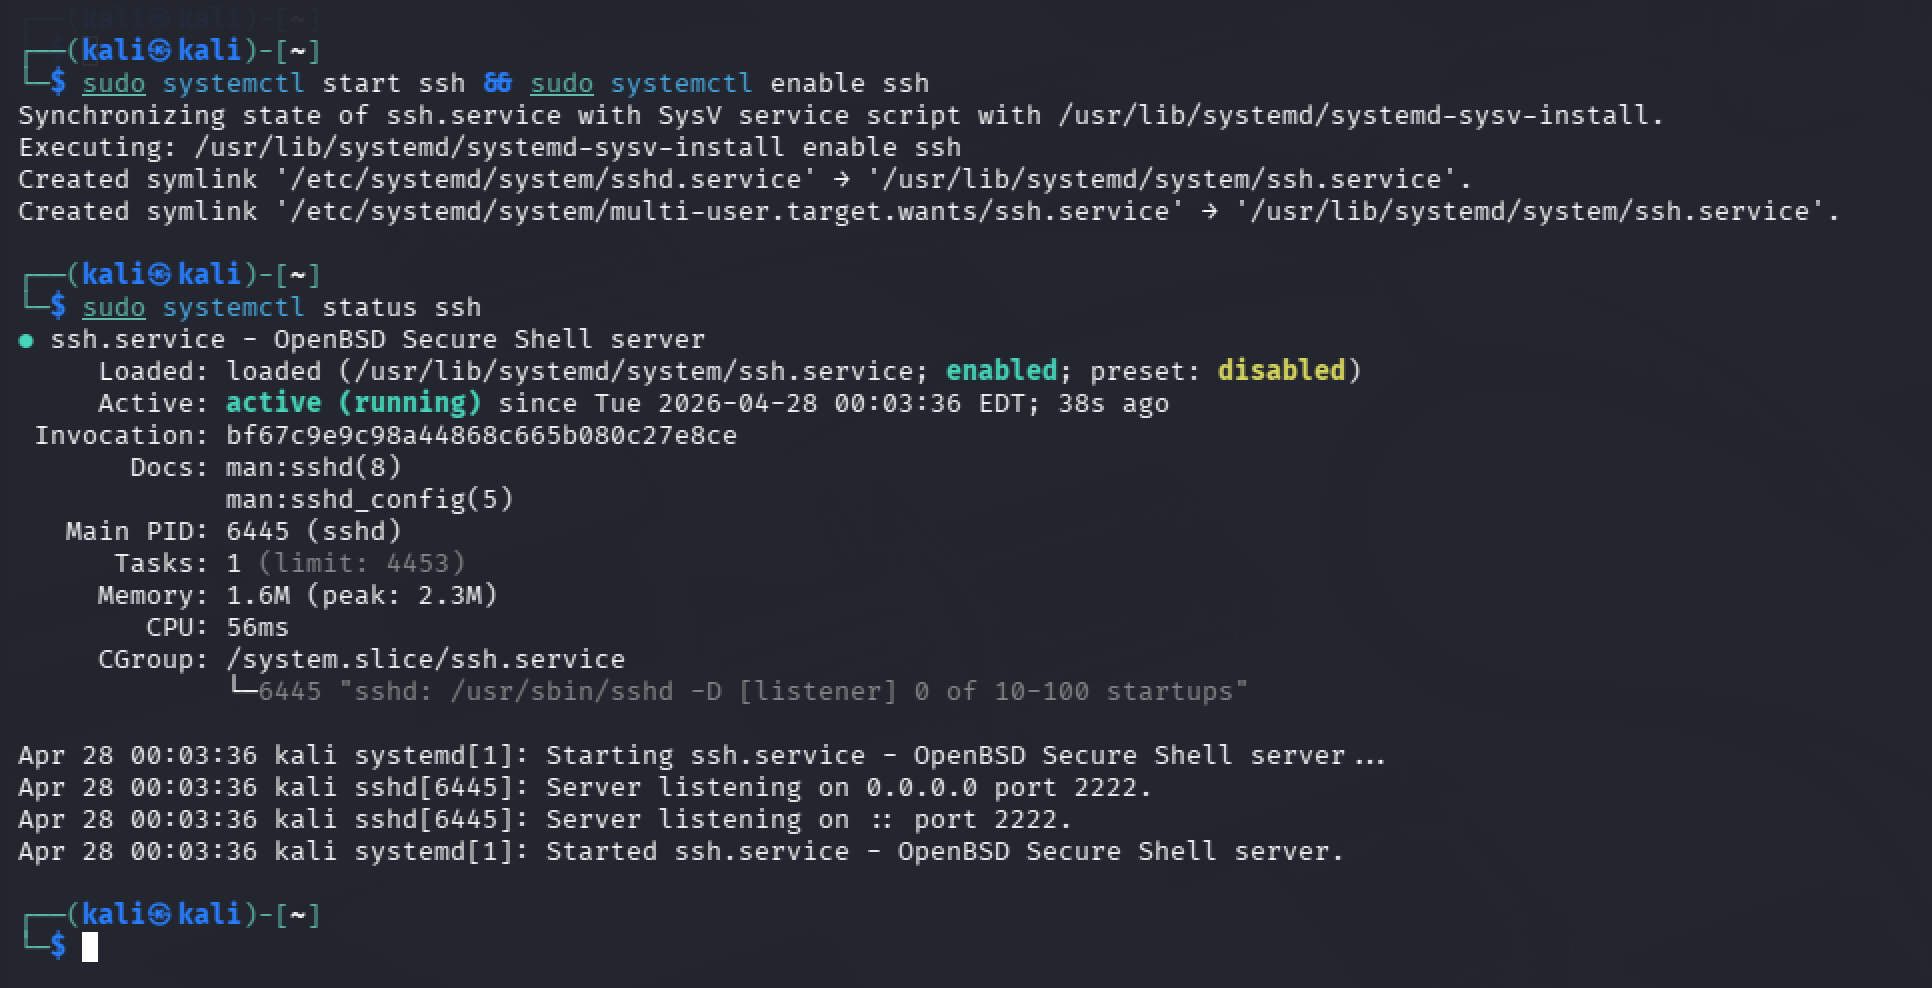
\includegraphics[width=0.85\textwidth]{imagenes/start_enable_ssh.png}
    \caption{Inicio y habilitación del servicio SSH en la VM de Kali Linux.}
    \label{fig:start-enable-ssh}
\end{figure}

En la imágen anterior simultáneamente se muestra el inicio del servicio SSH y su habilitación para que se inicie
automáticamente al arrancar la máquina. Luego, al hacer \texttt{systemctl status ssh} se muestra que el servicio
se encuentra activo y en ejecución en el puerto 2222.

\section{Cambio de puerto en la configuración de SSH}

\begin{figure}[H]
    \centering
    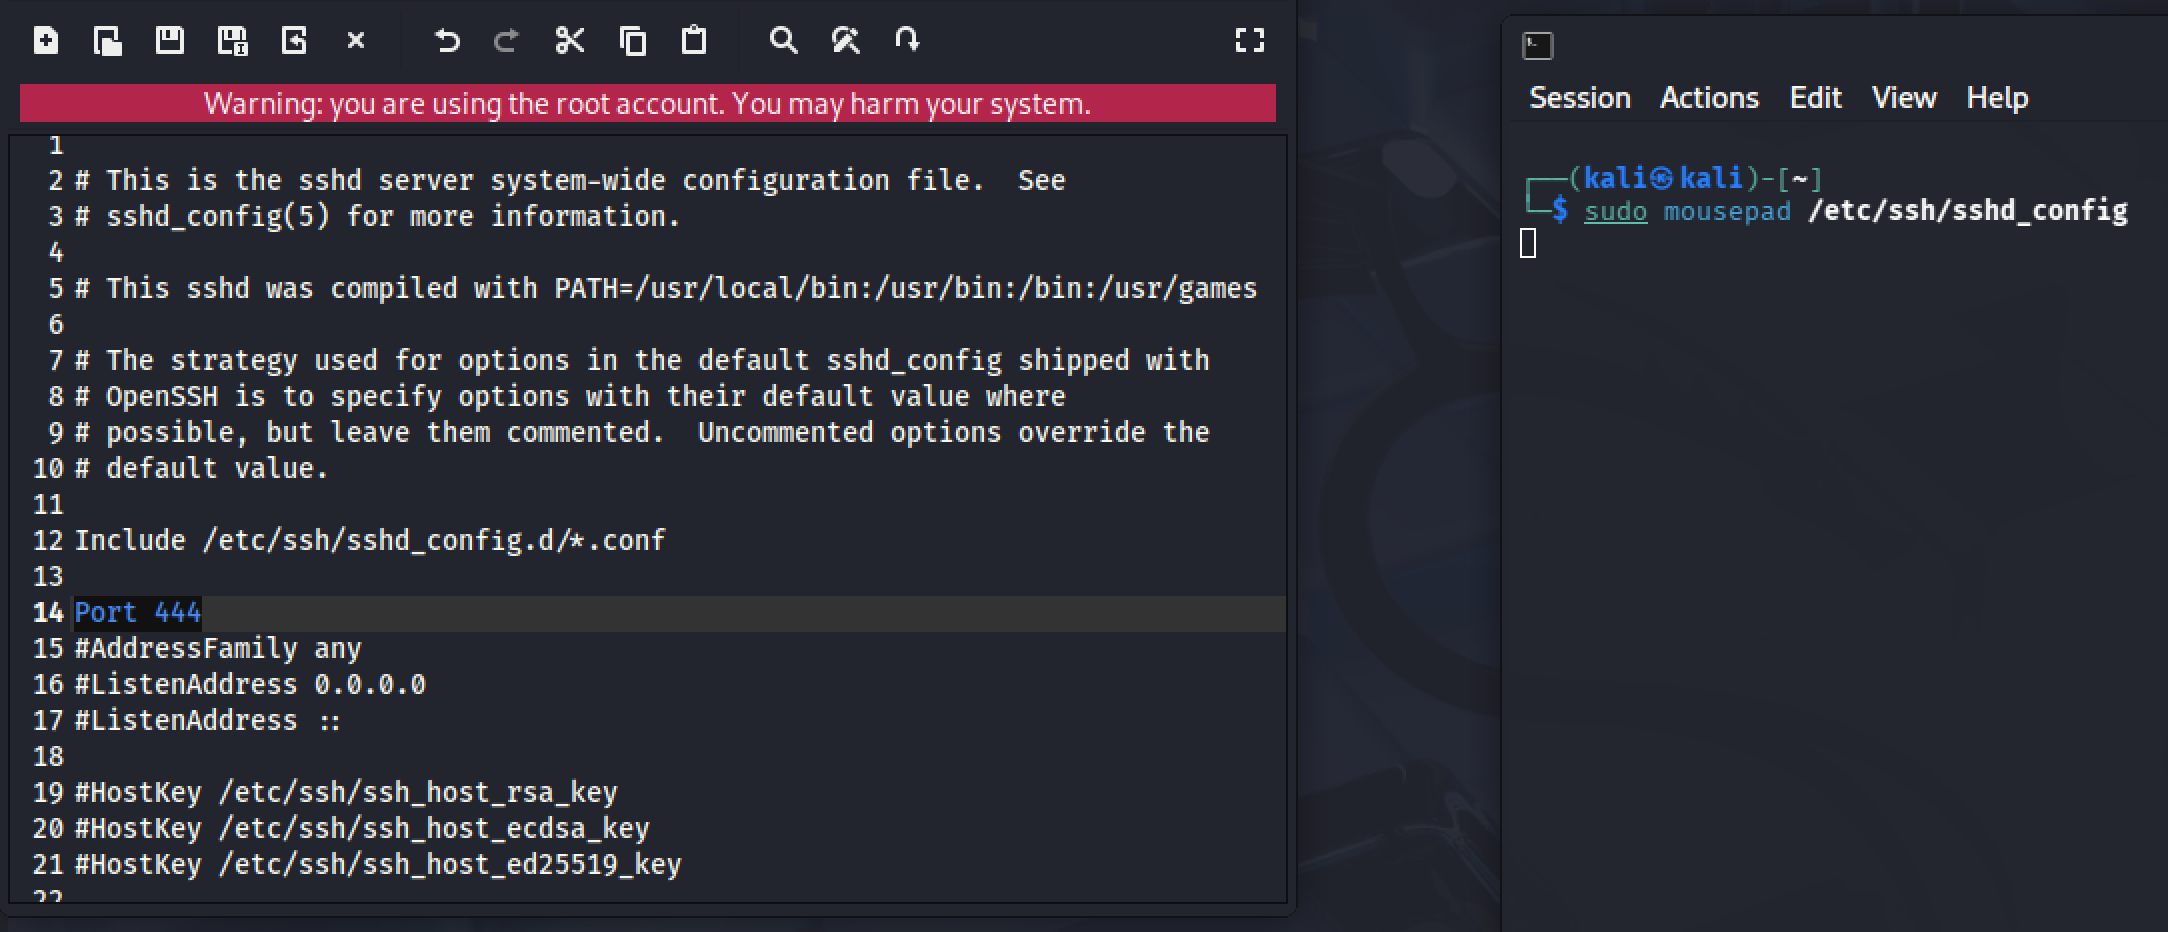
\includegraphics[width=0.85\textwidth]{imagenes/change_port_ssh.png}
    \caption{Cambio de puerto en la configuración sshd\_config.}
    \label{fig:change-port-ssh}
\end{figure}

Por gusto personal, en lugar de abrir \texttt{/etc/ssh/sshd\_config} con \texttt{nano}, usé el editor de texto
que viene integrado en la VM: \texttt{mousepad}. Luego, por elección personal, se cambió el puerto de escucha
al puerto 444.

Luego de modificar la configuración, se reinició el servicio SSH para que los cambios surtieran efecto. Al hacer
\texttt{systemctl status ssh} se muestra que el servicio se encuentra activo y en ejecución en el puerto 444.

\begin{figure}[H]
    \centering
    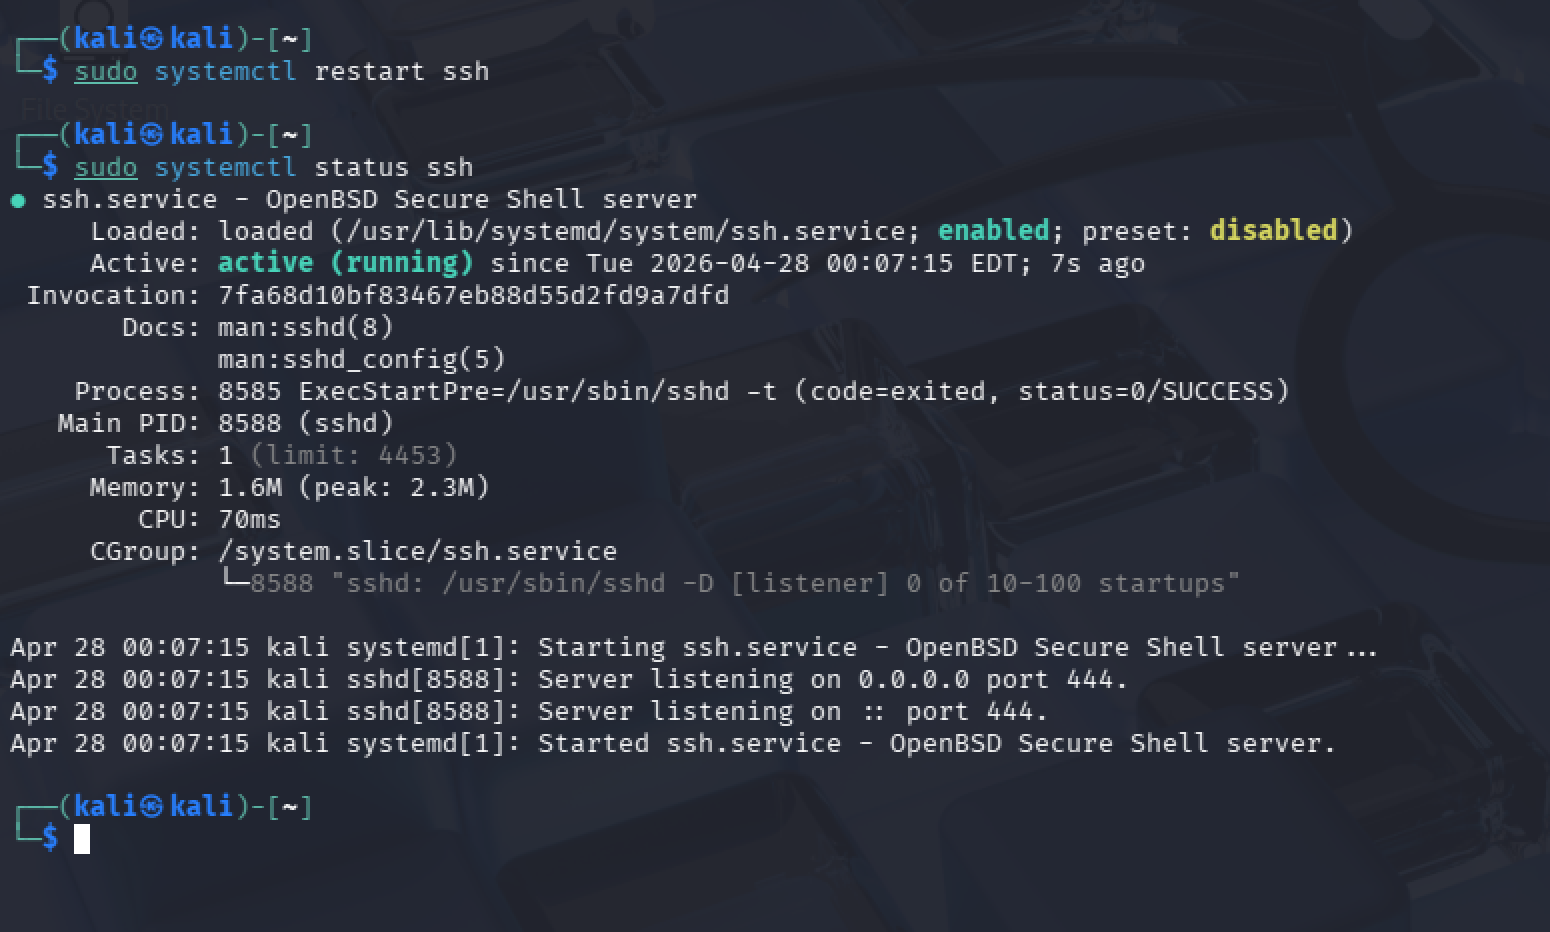
\includegraphics[width=0.85\textwidth]{imagenes/restart_ssh.png}
    \caption{Reinicio del servicio SSH después de modificar la configuración.}
    \label{fig:restart-ssh}
\end{figure}

\section{Conexión a la VM de Kali Linux desde la máquina Host}

Finalmente, para conectarnos a la VM de Kali Linux desde la máquina Host, se usó el comando \texttt{ssh} especificando
el puerto 444 y la dirección IP de la VM. Al ejecutar el comando, se solicitó la contraseña del usuario \texttt{kali}
y al ingresarla correctamente, se estableció la conexión SSH con éxito.

Nuestra forma de comprobación de que la conexión se estableció correctamente fue ejecutando el comando \texttt{fastfetch}
tanto en la máquina Host como en la VM de Kali Linux, y viendo los mismos resultados.

\begin{figure}[H]
    \centering
    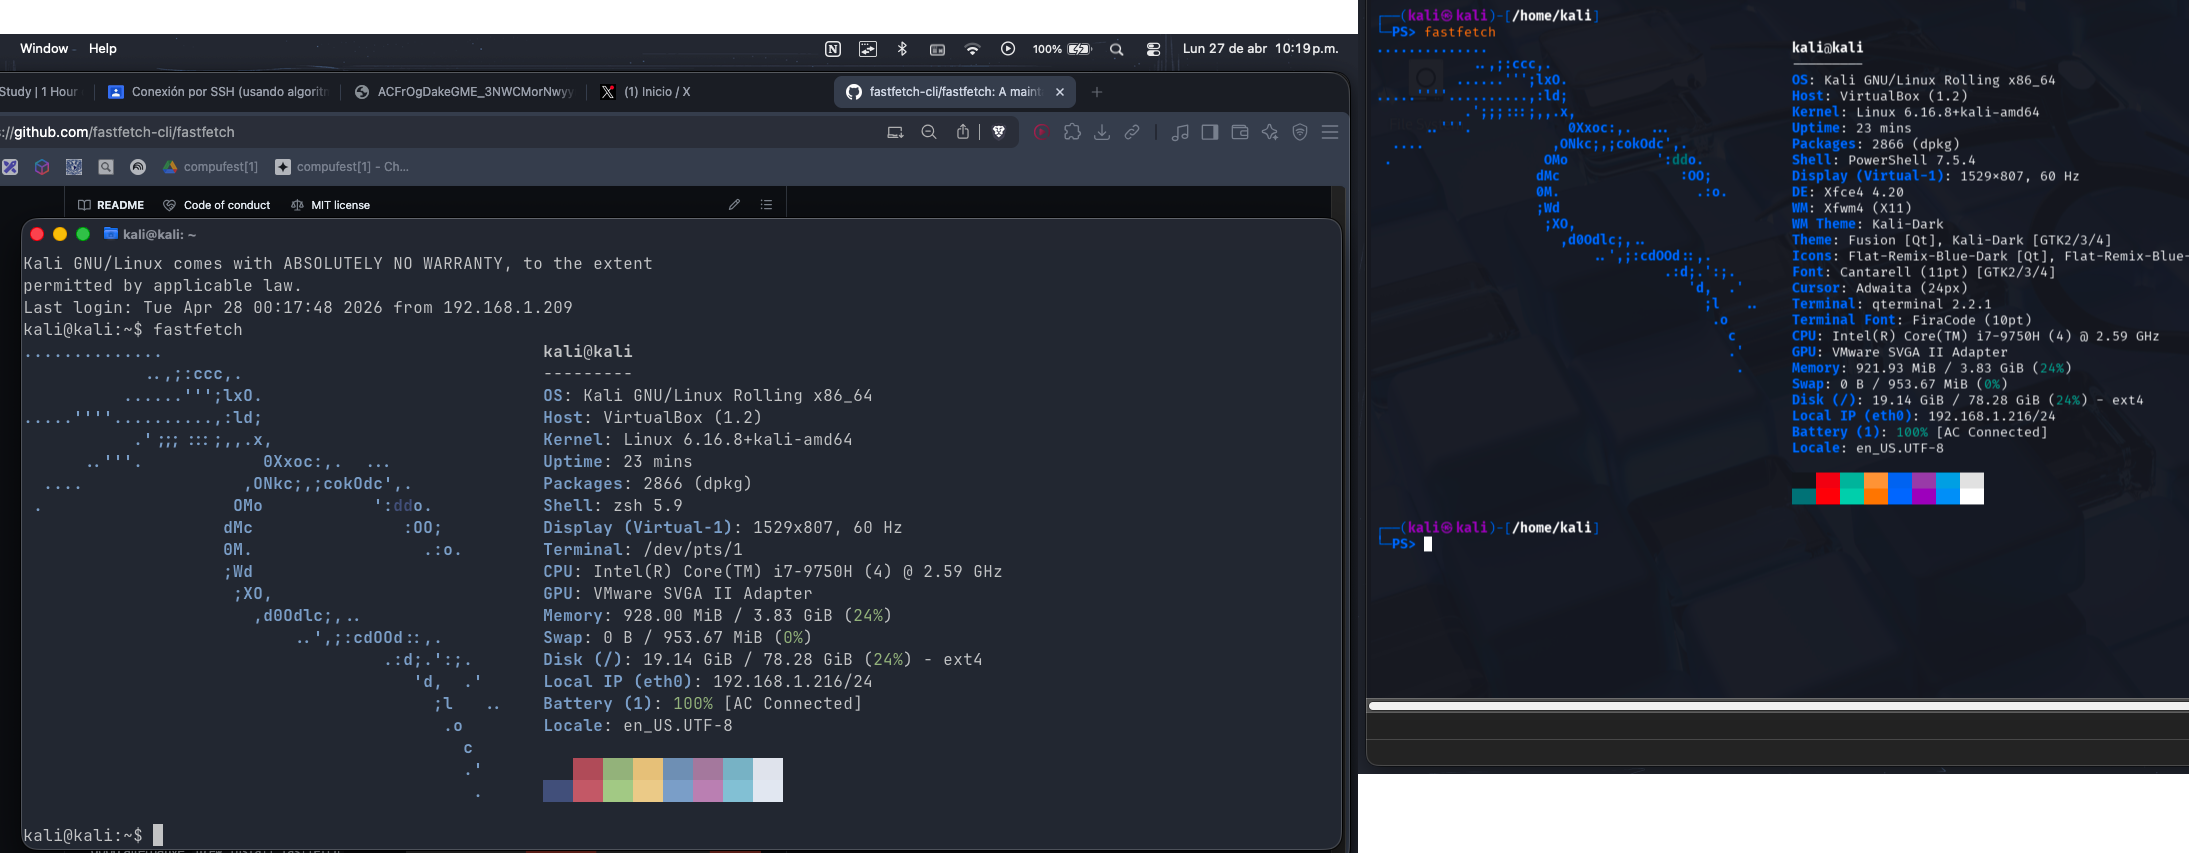
\includegraphics[width=0.85\textwidth]{imagenes/host_to_vm_ssh.png}
    \caption{Conexión a la VM de Kali desde la máquina Host.}
    \label{fig:ssh-host-to-vm}
\end{figure}

